% =============================================================================
% Section 3: Approach
% Structure mirrors "Diversifying Sequential Recommendation with Retrospective
% and Prospective Transformers" (Shi et al., TOIS 2024, Section 3):
%   3.1 Overview
%   3.2 Sequence Encoder (Embedding / Self-Attention)
%   3.3 Retrospective Greedy Search  (RT module)
%   3.4 Prospective Diversity Promoting (PT module)
%   3.5 Dense Next-Item Supervision
%   3.6 Diversity Promoting Loss
%   3.7 Type-Enriched Item Representations
% =============================================================================

\section{Approach}
\label{sec:approach}

\subsection{Overview}
\label{sec:overview}
We first state the model as a complete input--output system rather than as a set of modifications to an existing recommender. Given a user's chronologically ordered interaction sequence $S_u = (i_1, i_2, \dots, i_T)$ and the content metadata of the items (their semantic categories, and optionally creator and music tags), PACER produces two outputs: a relevance distribution $P_{\mathrm{rel}}(j \mid S_u)$ over the full item catalog $\mathcal{I}$ for the next interaction, and an ordered top-$k$ recommendation list $Y_u = (j_1, j_2, \dots, j_k)$ constructed from that distribution. The list must satisfy two requirements simultaneously: \emph{accuracy}, meaning its items are ones the user will actually engage with, and \emph{local diversity}, meaning adjacent items in the order of consumption are heterogeneous---the list must avoid long runs of same-category or near-duplicate content even when its set of items is already diverse. The architecture is organized around two modules that deliver these two requirements, a \textbf{Content} module and an \textbf{Order} module, as illustrated in Figure~\ref{fig:pacer_framework}.

Both modules operate over a shared two-stage transformer backbone built on the retrospective--prospective architecture of TRIER~\cite{shi2024trier}. A retrospective transformer (RT; Section~\ref{sec:rt}), trained as a reverse-direction sequence model, reconstructs plausible prefix interactions that could have preceded the observed history; beam search yields $M$ augmented views, each treated as one plausible latent intent of the user. A prospective transformer (PT; Section~\ref{sec:encoder}) encodes the observed sequence with causal forward attention and performs all recommendation scoring. On this backbone, the two modules have a clean division of responsibility: the Content module defines \emph{what items are}, the Order module defines \emph{where items are placed} in the output list.

The \textbf{Content} module (Section~\ref{sec:type_embeddings}) replaces identifier-only item representations with content-enriched ones. Every item is encoded at the input by the sum of its ID embedding, positional embedding, and a learnable type embedding pooled over its semantic categories, and the same type contribution is added to the output scoring matrix used for next-item ranking. Since the diversity objectives are defined in category space, this aligns the representation geometry the encoder learns with the geometry in which diversity is measured; creator and music channels enter through the identical mechanism in our embedding ablation. Training additionally supervises next-item prediction at every sequence position (Section~\ref{sec:dense}), sharpening the relevance distribution that the Order module starts from.

The \textbf{Order} module (Sections~\ref{sec:pt}--\ref{sec:diversity}) makes diversity a property of list order rather than of the list as a set. At each training step the prospective encoder decodes two lists in parallel, a relevance-only greedy list and a diverse list, with the RT views exposing the user's multiple intents. The diverse list is assembled step by step with a score combining three signals: relevance, a global intent-coverage term that down-weights intents already served by the chosen prefix, and a strictly local, position-aware term that penalizes candidates similar to the item placed at the immediately preceding position. A dual-path diversity loss rewards the additional diversity only in proportion to the likelihood it costs, and an optional consecutive-similarity loss directly discourages adjacent duplicates. At inference the same step-wise decoder runs with a relevance--coverage coefficient $\lambda$ and a consecutive coefficient $\lambda_c$, so a single trained model exposes a controllable accuracy--diversity operating point without retraining.

The remainder of this section presents the shared sequence encoder (Section~\ref{sec:encoder}) and the retrospective stage (Section~\ref{sec:rt}), then develops the Order module---prospective decoding, dense supervision, and its training objectives (Sections~\ref{sec:pt}--\ref{sec:diversity})---and finally details the Content module (Section~\ref{sec:type_embeddings}).

% Requires \usepackage{tikz} in the main preamble.
% =============================================================================
% PACER framework figure (self-contained TikZ; only requires \usepackage{tikz}
% in the main preamble). Components are grounded in the implementation:
%   - RT  : TRIER_RT reverse transformer, trained first, frozen during PT
%   - fuse: item + type(masked-mean category) + author + music + position
%   - PT  : forward transformer with dense per-position CE + cross-view NCE
%   - gen : step-wise top-k generation; greedy P_rel vs diverse
%           (1-lambda)P_rel + lambda P_cov paths (TRAINING paths shared by
%           L_div); NO lambda_c term here.
%   - sco : INFERENCE-only selection score S_s(j); this is the sole node that
%           carries the hard adjacent penalty -lambda_c C_s(j).
%   - losses: L_ce (dense), L_nce, L_div (ILD advantage),
%             gamma_o L_order (soft adjacent order, TRAINING only).
%   Routing rule: solid arrows = inference branch (sco -> R lists);
%   dashed arrows = training branch; the two never share an edge.
%
% LAYOUT NOTE: node minimum widths MUST be at least as wide as their longest
% text line. TikZ silently grows narrower nodes, sliding their west anchor
% left so neighbours overlap and arrows then point "backwards". If a box text
% changes, re-check its width (compile + render) before trusting the arrows.
%
% Input this file from approach.tex with % =============================================================================
% PACER framework figure (self-contained TikZ; only requires \usepackage{tikz}
% in the main preamble). Components are grounded in the implementation:
%   - RT  : TRIER_RT reverse transformer, trained first, frozen during PT
%   - fuse: item + type(masked-mean category) + author + music + position
%   - PT  : forward transformer with dense per-position CE + cross-view NCE
%   - gen : step-wise top-k generation; greedy P_rel vs diverse
%           (1-lambda)P_rel + lambda P_cov paths (TRAINING paths shared by
%           L_div); NO lambda_c term here.
%   - sco : INFERENCE-only selection score S_s(j); this is the sole node that
%           carries the hard adjacent penalty -lambda_c C_s(j).
%   - losses: L_ce (dense), L_nce, L_div (ILD advantage),
%             gamma_o L_order (soft adjacent order, TRAINING only).
%   Routing rule: solid arrows = inference branch (sco -> R lists);
%   dashed arrows = training branch; the two never share an edge.
%
% LAYOUT NOTE: node minimum widths MUST be at least as wide as their longest
% text line. TikZ silently grows narrower nodes, sliding their west anchor
% left so neighbours overlap and arrows then point "backwards". If a box text
% changes, re-check its width (compile + render) before trusting the arrows.
%
% Input this file from approach.tex with % =============================================================================
% PACER framework figure (self-contained TikZ; only requires \usepackage{tikz}
% in the main preamble). Components are grounded in the implementation:
%   - RT  : TRIER_RT reverse transformer, trained first, frozen during PT
%   - fuse: item + type(masked-mean category) + author + music + position
%   - PT  : forward transformer with dense per-position CE + cross-view NCE
%   - gen : step-wise top-k generation; greedy P_rel vs diverse
%           (1-lambda)P_rel + lambda P_cov paths (TRAINING paths shared by
%           L_div); NO lambda_c term here.
%   - sco : INFERENCE-only selection score S_s(j); this is the sole node that
%           carries the hard adjacent penalty -lambda_c C_s(j).
%   - losses: L_ce (dense), L_nce, L_div (ILD advantage),
%             gamma_o L_order (soft adjacent order, TRAINING only).
%   Routing rule: solid arrows = inference branch (sco -> R lists);
%   dashed arrows = training branch; the two never share an edge.
%
% LAYOUT NOTE: node minimum widths MUST be at least as wide as their longest
% text line. TikZ silently grows narrower nodes, sliding their west anchor
% left so neighbours overlap and arrows then point "backwards". If a box text
% changes, re-check its width (compile + render) before trusting the arrows.
%
% Input this file from approach.tex with \input{figures/pacer_framework.tex}.
% =============================================================================
\usetikzlibrary{arrows.meta,positioning,fit,backgrounds}

% Float placement notes (two-column):
%  - [t!] overrides LaTeX's aesthetic limits so the spanning float can take
%    the top of the *next* page even when tall.
%  - Preamble (main .tex), recommended:
%      \usepackage{dblfloatfix}                 % allow current-page placement
%      \usepackage{placeins}                    % \FloatBarrier support
%      \renewcommand{\dbltopfraction}{0.95}
%      \renewcommand{\dblfloatpagefraction}{0.7}
%  - To stop it drifting past a section, put \FloatBarrier where it must be
%    printed by (e.g. right before the next \subsection).
%  - Exact "on this page, right here" needs a non-float: use the strip
%    environment of the cuted package instead of figure*.
\begin{figure*}[t!]
\centering
% Overall size knob: fraction of the (two-column-spanning) \textwidth.
%   1.0\textwidth = full span (current); 0.8/0.7 = smaller, auto-centred.
% For a one-column figure: change figure* -> figure and use \columnwidth here.
% Prefer 0.85-1.0: below ~0.7 the scaled math/labels get hard to read; in that
% case shrink internals instead (font=\footnotesize, smaller node dimensions).
\resizebox{0.9\textwidth}{!}{%
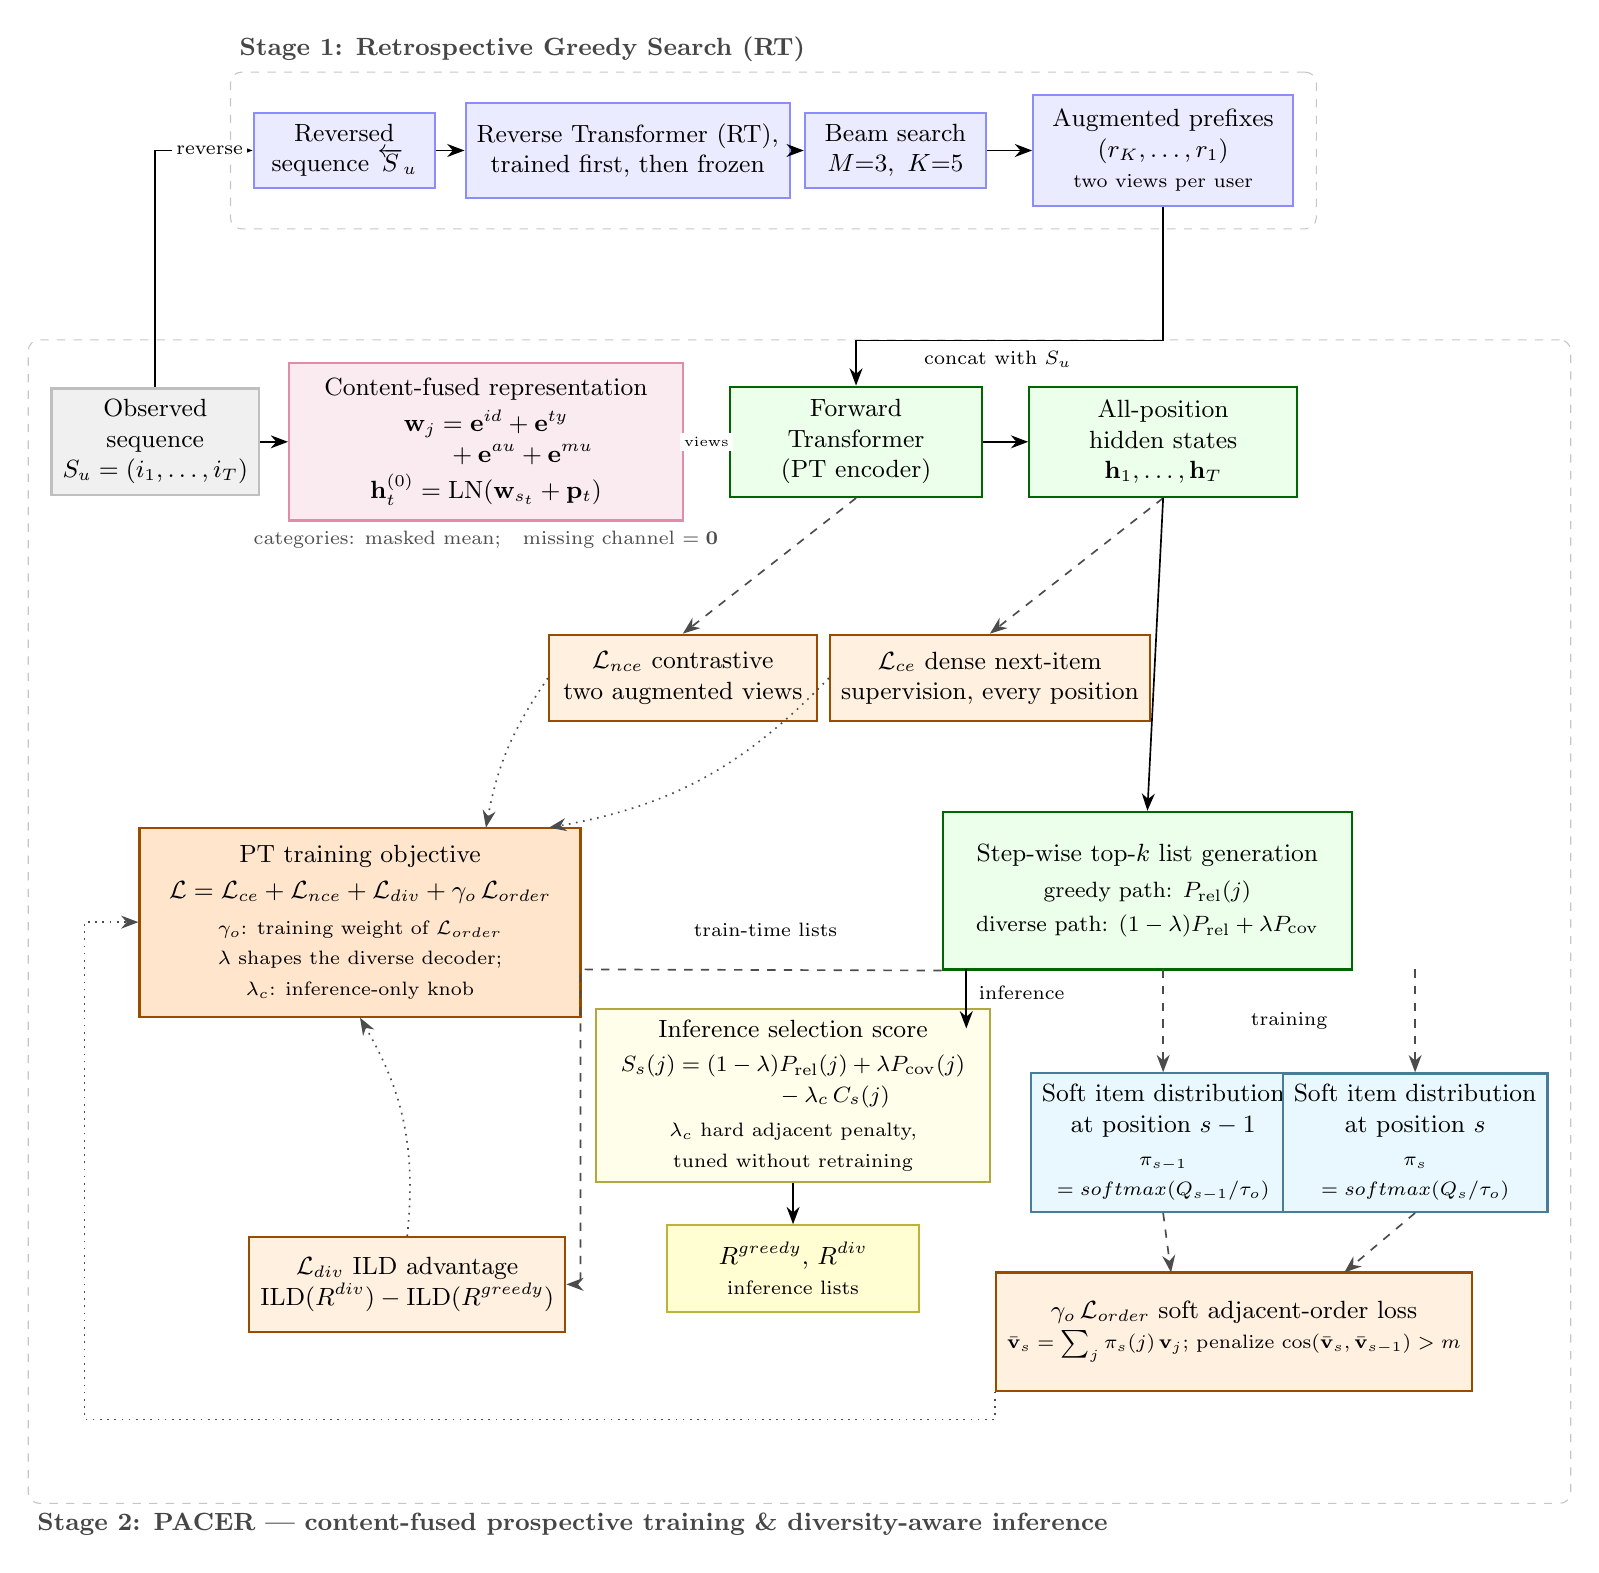
\begin{tikzpicture}[
  font=\small,
  box/.style={draw, align=center, inner sep=4pt,
              minimum height=0.95cm, thick},
  data/.style={box, fill=gray!12, draw=gray!50},
  rtb/.style={box, fill=blue!8, draw=blue!45},
  ptb/.style={box, fill=green!8, draw=green!40!black},
  emb/.style={box, fill=purple!8, draw=purple!45},
  loss/.style={box, fill=orange!12, draw=orange!60!black},
  softd/.style={box, fill=cyan!9, draw=cyan!55!black},
  lst/.style={box, fill=yellow!18, draw=yellow!70!black},
  scb/.style={box, fill=yellow!8, draw=yellow!65!black},
  arr/.style={-{Stealth[length=2.2mm]}, semithick},
  darr/.style={arr, dashed, gray!60!black},
  lbl/.style={font=\scriptsize, fill=white, inner sep=1.5pt},
  note/.style={font=\scriptsize, text=gray!60!black, align=center},
  stage/.style={draw=gray!45, dashed, rounded corners=4pt, inner sep=8pt},
  stagelbl/.style={font=\small\bfseries, text=gray!55!black}
]

% ---------------- main forward pipeline (y = 3.5) ----------------
\node[data, minimum width=2.6cm] (seq) at (0,3.5)
  {Observed\\ sequence\\ $S_u=(i_1,\ldots,i_T)$};

\node[emb, minimum width=5.0cm, minimum height=2.0cm] (fuse) at (4.2,3.5)
  {Content-fused representation\\[2pt]
   $\mathbf w_j=\mathbf e^{id}+\mathbf e^{ty}$\\
   $\phantom{\mathbf w_j=}\ +\mathbf e^{au}+\mathbf e^{mu}$\\[1pt]
   $\mathbf h_t^{(0)}=\mathrm{LN}(\mathbf w_{s_t}+\mathbf p_t)$};
\node[note, anchor=north] (fusenote) at (fuse.south)
  {categories: masked mean;\quad missing channel $=\mathbf 0$};

\node[ptb, minimum width=3.2cm, minimum height=1.4cm] (pte) at (8.9,3.5)
  {Forward\\ Transformer\\ (PT encoder)};

\node[ptb, minimum width=3.4cm, minimum height=1.4cm] (hs) at (12.8,3.5)
  {All-position\\ hidden states\\ $\mathbf h_1,\ldots,\mathbf h_T$};

\draw[arr] (seq.east) -- (fuse.west);
\draw[arr] (fuse.east) -- node[lbl, font=\tiny]{views} (pte.west);
\draw[arr] (pte.east) -- (hs.west);

% ---------------- Stage 1: RT (y = 7.2) ----------------
\node[rtb, minimum width=2.3cm] (rev) at (2.4,7.2)
  {Reversed\\ sequence $\overleftarrow S_u$};
\node[rtb, minimum width=3.2cm, minimum height=1.2cm] (rte) at (6.0,7.2)
  {Reverse Transformer (RT),\\ trained first, then frozen};
\node[rtb, minimum width=2.3cm] (beam) at (9.4,7.2)
  {Beam search\\ $M{=}3,\ K{=}5$};
\node[rtb, minimum width=3.3cm, minimum height=1.4cm] (pref) at (12.8,7.2)
  {Augmented prefixes\\ $(r_K,\ldots,r_1)$\\ {\scriptsize two views per user}};

\draw[arr] (seq.north) |- node[lbl, pos=0.78]{reverse} (rev.west);
\draw[arr] (rev.east) -- (rte.west);
\draw[arr] (rte.east) -- (beam.west);
\draw[arr] (beam.east) -- (pref.west);
% Route around the hidden-states box: down into the inter-row gap, then left,
% then into the top of the PT encoder.
\draw[arr] (pref.south) -- ++(0,-1.7) -| (pte.north);
\node[lbl] at (10.7,4.55) {concat with $S_u$};

% ---------------- training losses (y = 0.5) ----------------
\node[loss, minimum width=3.4cm, minimum height=1.1cm] (lnce) at (6.7,0.5)
  {$\mathcal L_{nce}$ contrastive\\ two augmented views};
\node[loss, minimum width=3.4cm, minimum height=1.1cm] (lce) at (10.6,0.5)
  {$\mathcal L_{ce}$ dense next-item\\ supervision, every position};
\draw[darr] (pte.south) -- (lnce.north);
\draw[darr] (hs.south) -- (lce.north);

% ---------------- total objective (bottom left) ----------------
\node[loss, fill=orange!20, minimum width=5.6cm, minimum height=2.4cm] (ltot)
  at (2.6,-2.6)
  {PT training objective\\[2pt]
   $\mathcal L=\mathcal L_{ce}+\mathcal L_{nce}+\mathcal L_{div}
    +\gamma_o\,\mathcal L_{order}$\\[2pt]
   {\scriptsize $\gamma_o$: training weight of $\mathcal L_{order}$}\\
   {\scriptsize $\lambda$ shapes the diverse decoder;}\\
   {\scriptsize $\lambda_c$: inference-only knob}};
% Both per-step losses feed the objective across its TOP edge, at distinct
% points, keeping the thin corridor UNDER the box (y=-3.2) completely clear.
\draw[darr, dotted] (lnce.west) to[bend right=12] (4.2,-1.4);
\draw[darr, dotted] (lce.west)  to[bend left=18]  (5.0,-1.4);

% ---------------- step-wise generation (right, y = -2.2) ----------------
% TRAINING-time generation: relevance path + diversity coverage path only.
% The hard adjacent penalty -lambda_c C_s(j) does NOT live here; it is applied
% exclusively in the inference selection-score node on the solid branch.
\node[ptb, minimum width=5.2cm, minimum height=2.0cm] (gen) at (12.6,-2.2)
  {Step-wise top-$k$ list generation\\[2pt]
   {\footnotesize greedy path: $P_{\mathrm{rel}}(j)$}\\[1pt]
   {\footnotesize diverse path:
    $(1-\lambda)P_{\mathrm{rel}}+\lambda P_{\mathrm{cov}}$}};
\draw[arr] (hs.south) -- (gen.north);

% ---------------- INFERENCE branch (SOLID): score then lists ---------------
% The FULL selection score, including -lambda_c C_s(j), exists only here.
\node[scb, minimum width=5.0cm, minimum height=1.7cm] (sco) at (8.1,-4.8)
  {Inference selection score\\[1.5pt]
   {\footnotesize $S_s(j)=(1-\lambda)P_{\mathrm{rel}}(j)
                       +\lambda P_{\mathrm{cov}}(j)$}\\
   {\footnotesize $\phantom{S_s(j)=}-\lambda_c\,C_s(j)$}\\[1.5pt]
   {\scriptsize $\lambda_c$ hard adjacent penalty,}\\
   {\scriptsize tuned without retraining}};
% Pure deployment output: this node has NO arrows into training losses.
\node[lst, minimum width=3.2cm, minimum height=1.1cm] (ri) at (8.1,-7.0)
  {$R^{greedy},\,R^{div}$\\ {\scriptsize inference lists}};
% Solid inference branch leaves gen just inside its SW corner and drops into
% the score node's north edge (short, entirely to the right of the score box).
\draw[arr] (10.3,-3.2) -- (10.3,-3.95);
\node[lbl, anchor=west] at (10.4,-3.5) {inference};
\draw[arr] (sco.south) -- (ri.north);

% ---------------- training-time soft distributions (DASHED branch) ----------
% The decoder scores Q_s at two adjacent positions are turned into soft item
% distributions; L_order reads BOTH of them (never an argmax'd token).
\node[softd, minimum width=3.0cm, minimum height=1.5cm] (pip) at (12.8,-5.4)
  {Soft item distribution\\ at position $s-1$\\[1pt]
   {\scriptsize $\boldsymbol\pi_{s-1}$}\\
   {\scriptsize $=\operatorname{softmax}(Q_{s-1}/\tau_o)$}};
\node[softd, minimum width=3.0cm, minimum height=1.5cm] (pi) at (16.0,-5.4)
  {Soft item distribution\\ at position $s$\\[1pt]
   {\scriptsize $\boldsymbol\pi_s$}\\
   {\scriptsize $=\operatorname{softmax}(Q_s/\tau_o)$}};
\draw[darr] (12.8,-3.2) -- (pip.north);
\draw[darr] (16.0,-3.2) -- (pi.north);
\node[lbl] at (14.4,-3.85) {training};

% ---------------- list-level training losses (bottom row) ------------------
\node[loss, minimum width=4.0cm, minimum height=1.2cm] (ldiv) at (3.2,-7.2)
  {$\mathcal L_{div}$ ILD advantage\\
   $\mathrm{ILD}(R^{div})-\mathrm{ILD}(R^{greedy})$};
\node[loss, minimum width=4.4cm, minimum height=1.5cm] (lo) at (13.7,-7.8)
  {$\gamma_o\,\mathcal L_{order}$ soft adjacent-order loss\\
   {\scriptsize $\bar{\mathbf v}_s=\sum_j \pi_s(j)\,\mathbf v_j$;
    penalize $\cos(\bar{\mathbf v}_s,\bar{\mathbf v}_{s-1})>m$}};

% Train-time list comparison: dashed, leaves the gen SW corner (the solid
% inference arrow leaves 0.3cm to its right), runs west through the clear
% corridor between objective (south -3.8) and score (north -3.95), drops in
% the gap between them, and enters L_div from the east.
\draw[darr] (gen.south west) -- (5.4,-3.2) -- (5.4,-7.2) -- (ldiv.east);
\node[lbl, anchor=north] at (7.75,-2.55) {train-time lists};

% The TWO ADJACENT SOFT DISTRIBUTIONS both point to L_order.
\draw[darr] (pip.south) -- (12.9,-7.05);
\draw[darr] (pi.south)  -- (15.1,-7.05);

% Losses roll up into the total training objective. L_div -> objective is a
% short curve on the left; L_order leaves from its SW corner along the BOTTOM
% corridor (below the inference lists and every loss box), rises in the
% far-left gap and enters the objective from the west.
\draw[darr, dotted] (ldiv.north) to[bend right=18] (ltot.south);
\draw[darr, dotted] (lo.south west) -- ++(0,-0.35) -| (-0.9,-2.6)
  -- (ltot.west);

% ---------------- stage frames ----------------
% pads keep the bottom/left L_order -> objective connector inside the frame.
\coordinate (framepad) at (8.5,-9.7);
\coordinate (framepadl) at (-1.1,-2.6);
\begin{scope}[on background layer]
  \node[stage, fit=(rev)(rte)(beam)(pref)] (st1) {};
  \node[stage, fit=(seq)(fuse)(fusenote)(pte)(hs)(lnce)(lce)(gen)
                       (sco)(ri)(pip)(pi)(ldiv)(lo)(ltot)
                       (framepad)(framepadl)] (st2) {};
\end{scope}
\node[stagelbl, anchor=south west] at (st1.north west)
  {Stage 1: Retrospective Greedy Search (RT)};
\node[stagelbl, anchor=north west] at (st2.south west)
  {Stage 2: PACER --- content-fused prospective training \& diversity-aware inference};

\end{tikzpicture}%
}
\caption{Overall PACER framework. \textbf{Stage 1 (RT):} a reverse-direction
transformer, trained independently and then frozen, hallucinates items that
could have preceded the observed sequence and returns beam-search augmented
views. \textbf{Stage 2 (PACER):} each item is represented by additive fusion of
ID, category (masked-mean pooled), creator, and music embeddings together with
a positional embedding; a forward transformer is trained with dense
per-position next-item supervision ($\mathcal L_{ce}$), cross-view contrastive
learning ($\mathcal L_{nce}$), an ILD list-diversity loss
($\mathcal L_{div}$), and a differentiable \emph{soft} adjacent-order loss
($\gamma_o\mathcal L_{order}$) computed from the soft item distributions at two
neighbouring list positions rather than from argmax tokens (solid arrows mark
the inference branch, dashed arrows the training branch). At inference, lists
are generated step by step with the combined relevance--coverage score that
additionally carries the hard adjacent-content penalty $-\lambda_c C_s(j)$;
$\lambda_c$ is tuned without retraining.}
\label{fig:pacer_framework}
\end{figure*}
.
% =============================================================================
\usetikzlibrary{arrows.meta,positioning,fit,backgrounds}

% Float placement notes (two-column):
%  - [t!] overrides LaTeX's aesthetic limits so the spanning float can take
%    the top of the *next* page even when tall.
%  - Preamble (main .tex), recommended:
%      \usepackage{dblfloatfix}                 % allow current-page placement
%      \usepackage{placeins}                    % \FloatBarrier support
%      \renewcommand{\dbltopfraction}{0.95}
%      \renewcommand{\dblfloatpagefraction}{0.7}
%  - To stop it drifting past a section, put \FloatBarrier where it must be
%    printed by (e.g. right before the next \subsection).
%  - Exact "on this page, right here" needs a non-float: use the strip
%    environment of the cuted package instead of figure*.
\begin{figure*}[t!]
\centering
% Overall size knob: fraction of the (two-column-spanning) \textwidth.
%   1.0\textwidth = full span (current); 0.8/0.7 = smaller, auto-centred.
% For a one-column figure: change figure* -> figure and use \columnwidth here.
% Prefer 0.85-1.0: below ~0.7 the scaled math/labels get hard to read; in that
% case shrink internals instead (font=\footnotesize, smaller node dimensions).
\resizebox{0.9\textwidth}{!}{%
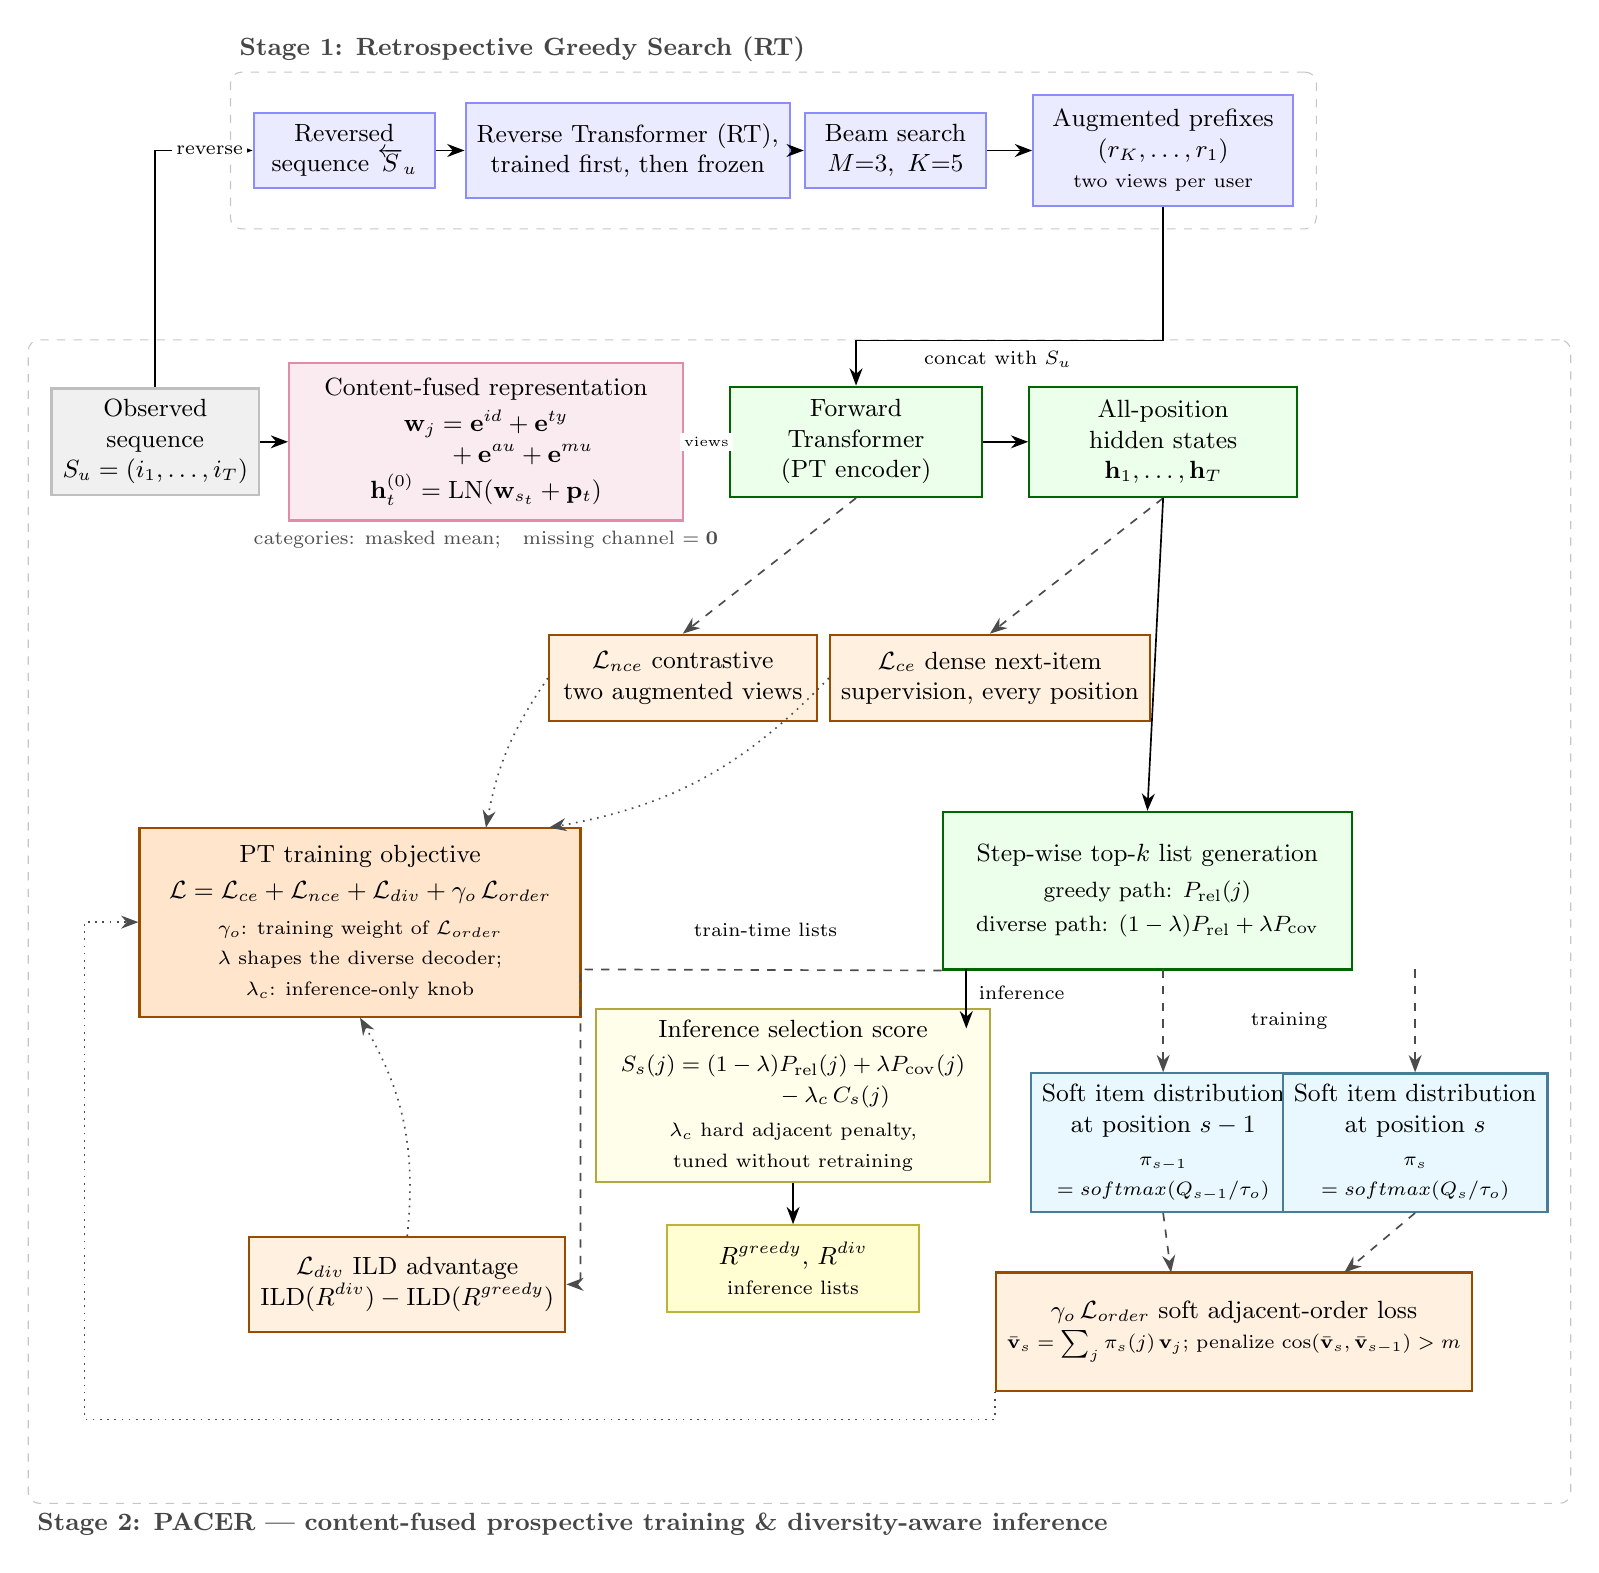
\begin{tikzpicture}[
  font=\small,
  box/.style={draw, align=center, inner sep=4pt,
              minimum height=0.95cm, thick},
  data/.style={box, fill=gray!12, draw=gray!50},
  rtb/.style={box, fill=blue!8, draw=blue!45},
  ptb/.style={box, fill=green!8, draw=green!40!black},
  emb/.style={box, fill=purple!8, draw=purple!45},
  loss/.style={box, fill=orange!12, draw=orange!60!black},
  softd/.style={box, fill=cyan!9, draw=cyan!55!black},
  lst/.style={box, fill=yellow!18, draw=yellow!70!black},
  scb/.style={box, fill=yellow!8, draw=yellow!65!black},
  arr/.style={-{Stealth[length=2.2mm]}, semithick},
  darr/.style={arr, dashed, gray!60!black},
  lbl/.style={font=\scriptsize, fill=white, inner sep=1.5pt},
  note/.style={font=\scriptsize, text=gray!60!black, align=center},
  stage/.style={draw=gray!45, dashed, rounded corners=4pt, inner sep=8pt},
  stagelbl/.style={font=\small\bfseries, text=gray!55!black}
]

% ---------------- main forward pipeline (y = 3.5) ----------------
\node[data, minimum width=2.6cm] (seq) at (0,3.5)
  {Observed\\ sequence\\ $S_u=(i_1,\ldots,i_T)$};

\node[emb, minimum width=5.0cm, minimum height=2.0cm] (fuse) at (4.2,3.5)
  {Content-fused representation\\[2pt]
   $\mathbf w_j=\mathbf e^{id}+\mathbf e^{ty}$\\
   $\phantom{\mathbf w_j=}\ +\mathbf e^{au}+\mathbf e^{mu}$\\[1pt]
   $\mathbf h_t^{(0)}=\mathrm{LN}(\mathbf w_{s_t}+\mathbf p_t)$};
\node[note, anchor=north] (fusenote) at (fuse.south)
  {categories: masked mean;\quad missing channel $=\mathbf 0$};

\node[ptb, minimum width=3.2cm, minimum height=1.4cm] (pte) at (8.9,3.5)
  {Forward\\ Transformer\\ (PT encoder)};

\node[ptb, minimum width=3.4cm, minimum height=1.4cm] (hs) at (12.8,3.5)
  {All-position\\ hidden states\\ $\mathbf h_1,\ldots,\mathbf h_T$};

\draw[arr] (seq.east) -- (fuse.west);
\draw[arr] (fuse.east) -- node[lbl, font=\tiny]{views} (pte.west);
\draw[arr] (pte.east) -- (hs.west);

% ---------------- Stage 1: RT (y = 7.2) ----------------
\node[rtb, minimum width=2.3cm] (rev) at (2.4,7.2)
  {Reversed\\ sequence $\overleftarrow S_u$};
\node[rtb, minimum width=3.2cm, minimum height=1.2cm] (rte) at (6.0,7.2)
  {Reverse Transformer (RT),\\ trained first, then frozen};
\node[rtb, minimum width=2.3cm] (beam) at (9.4,7.2)
  {Beam search\\ $M{=}3,\ K{=}5$};
\node[rtb, minimum width=3.3cm, minimum height=1.4cm] (pref) at (12.8,7.2)
  {Augmented prefixes\\ $(r_K,\ldots,r_1)$\\ {\scriptsize two views per user}};

\draw[arr] (seq.north) |- node[lbl, pos=0.78]{reverse} (rev.west);
\draw[arr] (rev.east) -- (rte.west);
\draw[arr] (rte.east) -- (beam.west);
\draw[arr] (beam.east) -- (pref.west);
% Route around the hidden-states box: down into the inter-row gap, then left,
% then into the top of the PT encoder.
\draw[arr] (pref.south) -- ++(0,-1.7) -| (pte.north);
\node[lbl] at (10.7,4.55) {concat with $S_u$};

% ---------------- training losses (y = 0.5) ----------------
\node[loss, minimum width=3.4cm, minimum height=1.1cm] (lnce) at (6.7,0.5)
  {$\mathcal L_{nce}$ contrastive\\ two augmented views};
\node[loss, minimum width=3.4cm, minimum height=1.1cm] (lce) at (10.6,0.5)
  {$\mathcal L_{ce}$ dense next-item\\ supervision, every position};
\draw[darr] (pte.south) -- (lnce.north);
\draw[darr] (hs.south) -- (lce.north);

% ---------------- total objective (bottom left) ----------------
\node[loss, fill=orange!20, minimum width=5.6cm, minimum height=2.4cm] (ltot)
  at (2.6,-2.6)
  {PT training objective\\[2pt]
   $\mathcal L=\mathcal L_{ce}+\mathcal L_{nce}+\mathcal L_{div}
    +\gamma_o\,\mathcal L_{order}$\\[2pt]
   {\scriptsize $\gamma_o$: training weight of $\mathcal L_{order}$}\\
   {\scriptsize $\lambda$ shapes the diverse decoder;}\\
   {\scriptsize $\lambda_c$: inference-only knob}};
% Both per-step losses feed the objective across its TOP edge, at distinct
% points, keeping the thin corridor UNDER the box (y=-3.2) completely clear.
\draw[darr, dotted] (lnce.west) to[bend right=12] (4.2,-1.4);
\draw[darr, dotted] (lce.west)  to[bend left=18]  (5.0,-1.4);

% ---------------- step-wise generation (right, y = -2.2) ----------------
% TRAINING-time generation: relevance path + diversity coverage path only.
% The hard adjacent penalty -lambda_c C_s(j) does NOT live here; it is applied
% exclusively in the inference selection-score node on the solid branch.
\node[ptb, minimum width=5.2cm, minimum height=2.0cm] (gen) at (12.6,-2.2)
  {Step-wise top-$k$ list generation\\[2pt]
   {\footnotesize greedy path: $P_{\mathrm{rel}}(j)$}\\[1pt]
   {\footnotesize diverse path:
    $(1-\lambda)P_{\mathrm{rel}}+\lambda P_{\mathrm{cov}}$}};
\draw[arr] (hs.south) -- (gen.north);

% ---------------- INFERENCE branch (SOLID): score then lists ---------------
% The FULL selection score, including -lambda_c C_s(j), exists only here.
\node[scb, minimum width=5.0cm, minimum height=1.7cm] (sco) at (8.1,-4.8)
  {Inference selection score\\[1.5pt]
   {\footnotesize $S_s(j)=(1-\lambda)P_{\mathrm{rel}}(j)
                       +\lambda P_{\mathrm{cov}}(j)$}\\
   {\footnotesize $\phantom{S_s(j)=}-\lambda_c\,C_s(j)$}\\[1.5pt]
   {\scriptsize $\lambda_c$ hard adjacent penalty,}\\
   {\scriptsize tuned without retraining}};
% Pure deployment output: this node has NO arrows into training losses.
\node[lst, minimum width=3.2cm, minimum height=1.1cm] (ri) at (8.1,-7.0)
  {$R^{greedy},\,R^{div}$\\ {\scriptsize inference lists}};
% Solid inference branch leaves gen just inside its SW corner and drops into
% the score node's north edge (short, entirely to the right of the score box).
\draw[arr] (10.3,-3.2) -- (10.3,-3.95);
\node[lbl, anchor=west] at (10.4,-3.5) {inference};
\draw[arr] (sco.south) -- (ri.north);

% ---------------- training-time soft distributions (DASHED branch) ----------
% The decoder scores Q_s at two adjacent positions are turned into soft item
% distributions; L_order reads BOTH of them (never an argmax'd token).
\node[softd, minimum width=3.0cm, minimum height=1.5cm] (pip) at (12.8,-5.4)
  {Soft item distribution\\ at position $s-1$\\[1pt]
   {\scriptsize $\boldsymbol\pi_{s-1}$}\\
   {\scriptsize $=\operatorname{softmax}(Q_{s-1}/\tau_o)$}};
\node[softd, minimum width=3.0cm, minimum height=1.5cm] (pi) at (16.0,-5.4)
  {Soft item distribution\\ at position $s$\\[1pt]
   {\scriptsize $\boldsymbol\pi_s$}\\
   {\scriptsize $=\operatorname{softmax}(Q_s/\tau_o)$}};
\draw[darr] (12.8,-3.2) -- (pip.north);
\draw[darr] (16.0,-3.2) -- (pi.north);
\node[lbl] at (14.4,-3.85) {training};

% ---------------- list-level training losses (bottom row) ------------------
\node[loss, minimum width=4.0cm, minimum height=1.2cm] (ldiv) at (3.2,-7.2)
  {$\mathcal L_{div}$ ILD advantage\\
   $\mathrm{ILD}(R^{div})-\mathrm{ILD}(R^{greedy})$};
\node[loss, minimum width=4.4cm, minimum height=1.5cm] (lo) at (13.7,-7.8)
  {$\gamma_o\,\mathcal L_{order}$ soft adjacent-order loss\\
   {\scriptsize $\bar{\mathbf v}_s=\sum_j \pi_s(j)\,\mathbf v_j$;
    penalize $\cos(\bar{\mathbf v}_s,\bar{\mathbf v}_{s-1})>m$}};

% Train-time list comparison: dashed, leaves the gen SW corner (the solid
% inference arrow leaves 0.3cm to its right), runs west through the clear
% corridor between objective (south -3.8) and score (north -3.95), drops in
% the gap between them, and enters L_div from the east.
\draw[darr] (gen.south west) -- (5.4,-3.2) -- (5.4,-7.2) -- (ldiv.east);
\node[lbl, anchor=north] at (7.75,-2.55) {train-time lists};

% The TWO ADJACENT SOFT DISTRIBUTIONS both point to L_order.
\draw[darr] (pip.south) -- (12.9,-7.05);
\draw[darr] (pi.south)  -- (15.1,-7.05);

% Losses roll up into the total training objective. L_div -> objective is a
% short curve on the left; L_order leaves from its SW corner along the BOTTOM
% corridor (below the inference lists and every loss box), rises in the
% far-left gap and enters the objective from the west.
\draw[darr, dotted] (ldiv.north) to[bend right=18] (ltot.south);
\draw[darr, dotted] (lo.south west) -- ++(0,-0.35) -| (-0.9,-2.6)
  -- (ltot.west);

% ---------------- stage frames ----------------
% pads keep the bottom/left L_order -> objective connector inside the frame.
\coordinate (framepad) at (8.5,-9.7);
\coordinate (framepadl) at (-1.1,-2.6);
\begin{scope}[on background layer]
  \node[stage, fit=(rev)(rte)(beam)(pref)] (st1) {};
  \node[stage, fit=(seq)(fuse)(fusenote)(pte)(hs)(lnce)(lce)(gen)
                       (sco)(ri)(pip)(pi)(ldiv)(lo)(ltot)
                       (framepad)(framepadl)] (st2) {};
\end{scope}
\node[stagelbl, anchor=south west] at (st1.north west)
  {Stage 1: Retrospective Greedy Search (RT)};
\node[stagelbl, anchor=north west] at (st2.south west)
  {Stage 2: PACER --- content-fused prospective training \& diversity-aware inference};

\end{tikzpicture}%
}
\caption{Overall PACER framework. \textbf{Stage 1 (RT):} a reverse-direction
transformer, trained independently and then frozen, hallucinates items that
could have preceded the observed sequence and returns beam-search augmented
views. \textbf{Stage 2 (PACER):} each item is represented by additive fusion of
ID, category (masked-mean pooled), creator, and music embeddings together with
a positional embedding; a forward transformer is trained with dense
per-position next-item supervision ($\mathcal L_{ce}$), cross-view contrastive
learning ($\mathcal L_{nce}$), an ILD list-diversity loss
($\mathcal L_{div}$), and a differentiable \emph{soft} adjacent-order loss
($\gamma_o\mathcal L_{order}$) computed from the soft item distributions at two
neighbouring list positions rather than from argmax tokens (solid arrows mark
the inference branch, dashed arrows the training branch). At inference, lists
are generated step by step with the combined relevance--coverage score that
additionally carries the hard adjacent-content penalty $-\lambda_c C_s(j)$;
$\lambda_c$ is tuned without retraining.}
\label{fig:pacer_framework}
\end{figure*}
.
% =============================================================================
\usetikzlibrary{arrows.meta,positioning,fit,backgrounds}

% Float placement notes (two-column):
%  - [t!] overrides LaTeX's aesthetic limits so the spanning float can take
%    the top of the *next* page even when tall.
%  - Preamble (main .tex), recommended:
%      \usepackage{dblfloatfix}                 % allow current-page placement
%      \usepackage{placeins}                    % \FloatBarrier support
%      \renewcommand{\dbltopfraction}{0.95}
%      \renewcommand{\dblfloatpagefraction}{0.7}
%  - To stop it drifting past a section, put \FloatBarrier where it must be
%    printed by (e.g. right before the next \subsection).
%  - Exact "on this page, right here" needs a non-float: use the strip
%    environment of the cuted package instead of figure*.
\begin{figure*}[t!]
\centering
% Overall size knob: fraction of the (two-column-spanning) \textwidth.
%   1.0\textwidth = full span (current); 0.8/0.7 = smaller, auto-centred.
% For a one-column figure: change figure* -> figure and use \columnwidth here.
% Prefer 0.85-1.0: below ~0.7 the scaled math/labels get hard to read; in that
% case shrink internals instead (font=\footnotesize, smaller node dimensions).
\resizebox{0.9\textwidth}{!}{%
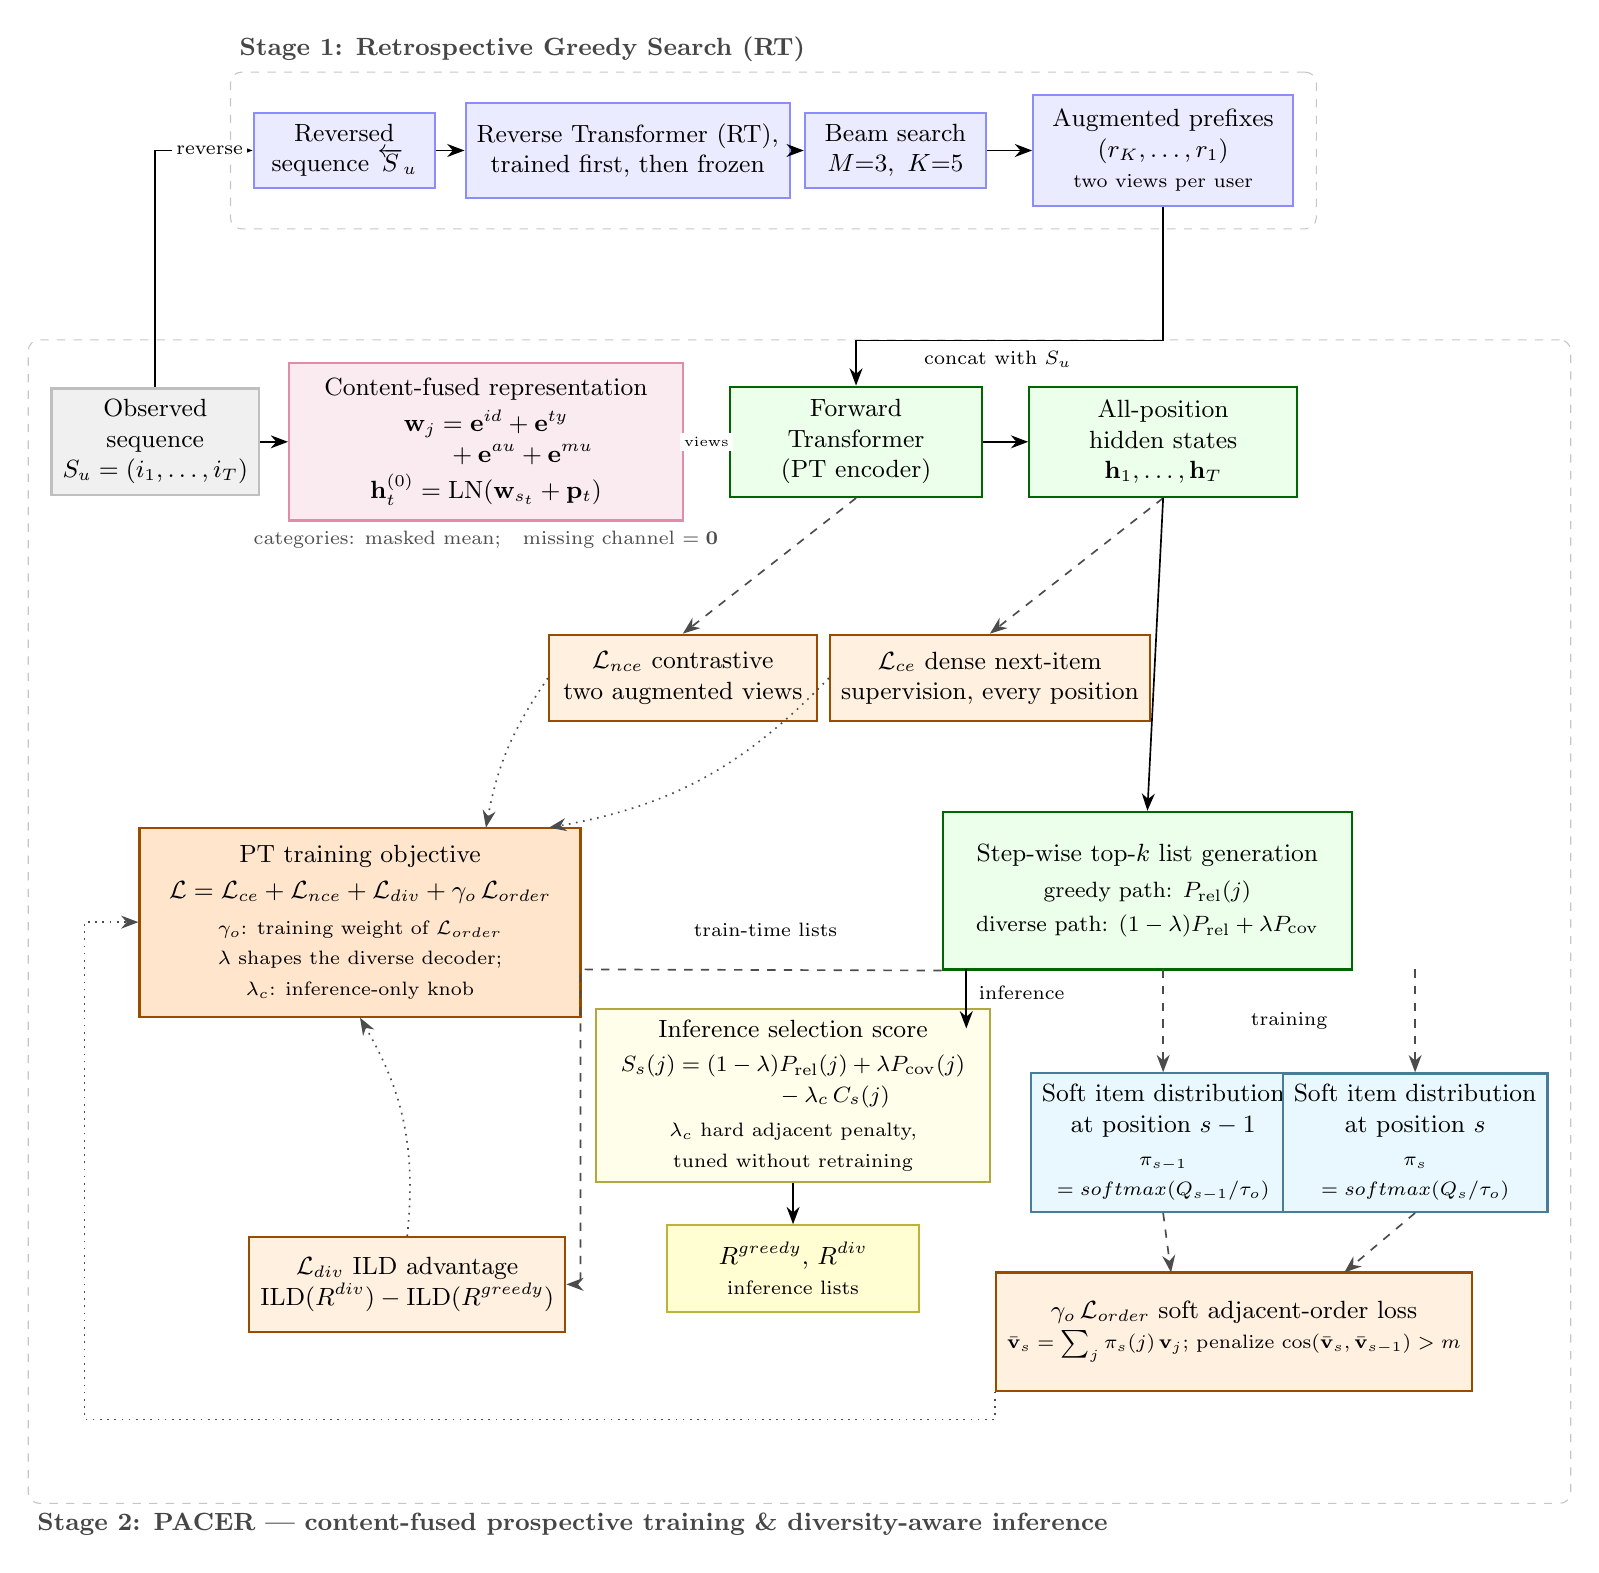
\begin{tikzpicture}[
  font=\small,
  box/.style={draw, align=center, inner sep=4pt,
              minimum height=0.95cm, thick},
  data/.style={box, fill=gray!12, draw=gray!50},
  rtb/.style={box, fill=blue!8, draw=blue!45},
  ptb/.style={box, fill=green!8, draw=green!40!black},
  emb/.style={box, fill=purple!8, draw=purple!45},
  loss/.style={box, fill=orange!12, draw=orange!60!black},
  softd/.style={box, fill=cyan!9, draw=cyan!55!black},
  lst/.style={box, fill=yellow!18, draw=yellow!70!black},
  scb/.style={box, fill=yellow!8, draw=yellow!65!black},
  arr/.style={-{Stealth[length=2.2mm]}, semithick},
  darr/.style={arr, dashed, gray!60!black},
  lbl/.style={font=\scriptsize, fill=white, inner sep=1.5pt},
  note/.style={font=\scriptsize, text=gray!60!black, align=center},
  stage/.style={draw=gray!45, dashed, rounded corners=4pt, inner sep=8pt},
  stagelbl/.style={font=\small\bfseries, text=gray!55!black}
]

% ---------------- main forward pipeline (y = 3.5) ----------------
\node[data, minimum width=2.6cm] (seq) at (0,3.5)
  {Observed\\ sequence\\ $S_u=(i_1,\ldots,i_T)$};

\node[emb, minimum width=5.0cm, minimum height=2.0cm] (fuse) at (4.2,3.5)
  {Content-fused representation\\[2pt]
   $\mathbf w_j=\mathbf e^{id}+\mathbf e^{ty}$\\
   $\phantom{\mathbf w_j=}\ +\mathbf e^{au}+\mathbf e^{mu}$\\[1pt]
   $\mathbf h_t^{(0)}=\mathrm{LN}(\mathbf w_{s_t}+\mathbf p_t)$};
\node[note, anchor=north] (fusenote) at (fuse.south)
  {categories: masked mean;\quad missing channel $=\mathbf 0$};

\node[ptb, minimum width=3.2cm, minimum height=1.4cm] (pte) at (8.9,3.5)
  {Forward\\ Transformer\\ (PT encoder)};

\node[ptb, minimum width=3.4cm, minimum height=1.4cm] (hs) at (12.8,3.5)
  {All-position\\ hidden states\\ $\mathbf h_1,\ldots,\mathbf h_T$};

\draw[arr] (seq.east) -- (fuse.west);
\draw[arr] (fuse.east) -- node[lbl, font=\tiny]{views} (pte.west);
\draw[arr] (pte.east) -- (hs.west);

% ---------------- Stage 1: RT (y = 7.2) ----------------
\node[rtb, minimum width=2.3cm] (rev) at (2.4,7.2)
  {Reversed\\ sequence $\overleftarrow S_u$};
\node[rtb, minimum width=3.2cm, minimum height=1.2cm] (rte) at (6.0,7.2)
  {Reverse Transformer (RT),\\ trained first, then frozen};
\node[rtb, minimum width=2.3cm] (beam) at (9.4,7.2)
  {Beam search\\ $M{=}3,\ K{=}5$};
\node[rtb, minimum width=3.3cm, minimum height=1.4cm] (pref) at (12.8,7.2)
  {Augmented prefixes\\ $(r_K,\ldots,r_1)$\\ {\scriptsize two views per user}};

\draw[arr] (seq.north) |- node[lbl, pos=0.78]{reverse} (rev.west);
\draw[arr] (rev.east) -- (rte.west);
\draw[arr] (rte.east) -- (beam.west);
\draw[arr] (beam.east) -- (pref.west);
% Route around the hidden-states box: down into the inter-row gap, then left,
% then into the top of the PT encoder.
\draw[arr] (pref.south) -- ++(0,-1.7) -| (pte.north);
\node[lbl] at (10.7,4.55) {concat with $S_u$};

% ---------------- training losses (y = 0.5) ----------------
\node[loss, minimum width=3.4cm, minimum height=1.1cm] (lnce) at (6.7,0.5)
  {$\mathcal L_{nce}$ contrastive\\ two augmented views};
\node[loss, minimum width=3.4cm, minimum height=1.1cm] (lce) at (10.6,0.5)
  {$\mathcal L_{ce}$ dense next-item\\ supervision, every position};
\draw[darr] (pte.south) -- (lnce.north);
\draw[darr] (hs.south) -- (lce.north);

% ---------------- total objective (bottom left) ----------------
\node[loss, fill=orange!20, minimum width=5.6cm, minimum height=2.4cm] (ltot)
  at (2.6,-2.6)
  {PT training objective\\[2pt]
   $\mathcal L=\mathcal L_{ce}+\mathcal L_{nce}+\mathcal L_{div}
    +\gamma_o\,\mathcal L_{order}$\\[2pt]
   {\scriptsize $\gamma_o$: training weight of $\mathcal L_{order}$}\\
   {\scriptsize $\lambda$ shapes the diverse decoder;}\\
   {\scriptsize $\lambda_c$: inference-only knob}};
% Both per-step losses feed the objective across its TOP edge, at distinct
% points, keeping the thin corridor UNDER the box (y=-3.2) completely clear.
\draw[darr, dotted] (lnce.west) to[bend right=12] (4.2,-1.4);
\draw[darr, dotted] (lce.west)  to[bend left=18]  (5.0,-1.4);

% ---------------- step-wise generation (right, y = -2.2) ----------------
% TRAINING-time generation: relevance path + diversity coverage path only.
% The hard adjacent penalty -lambda_c C_s(j) does NOT live here; it is applied
% exclusively in the inference selection-score node on the solid branch.
\node[ptb, minimum width=5.2cm, minimum height=2.0cm] (gen) at (12.6,-2.2)
  {Step-wise top-$k$ list generation\\[2pt]
   {\footnotesize greedy path: $P_{\mathrm{rel}}(j)$}\\[1pt]
   {\footnotesize diverse path:
    $(1-\lambda)P_{\mathrm{rel}}+\lambda P_{\mathrm{cov}}$}};
\draw[arr] (hs.south) -- (gen.north);

% ---------------- INFERENCE branch (SOLID): score then lists ---------------
% The FULL selection score, including -lambda_c C_s(j), exists only here.
\node[scb, minimum width=5.0cm, minimum height=1.7cm] (sco) at (8.1,-4.8)
  {Inference selection score\\[1.5pt]
   {\footnotesize $S_s(j)=(1-\lambda)P_{\mathrm{rel}}(j)
                       +\lambda P_{\mathrm{cov}}(j)$}\\
   {\footnotesize $\phantom{S_s(j)=}-\lambda_c\,C_s(j)$}\\[1.5pt]
   {\scriptsize $\lambda_c$ hard adjacent penalty,}\\
   {\scriptsize tuned without retraining}};
% Pure deployment output: this node has NO arrows into training losses.
\node[lst, minimum width=3.2cm, minimum height=1.1cm] (ri) at (8.1,-7.0)
  {$R^{greedy},\,R^{div}$\\ {\scriptsize inference lists}};
% Solid inference branch leaves gen just inside its SW corner and drops into
% the score node's north edge (short, entirely to the right of the score box).
\draw[arr] (10.3,-3.2) -- (10.3,-3.95);
\node[lbl, anchor=west] at (10.4,-3.5) {inference};
\draw[arr] (sco.south) -- (ri.north);

% ---------------- training-time soft distributions (DASHED branch) ----------
% The decoder scores Q_s at two adjacent positions are turned into soft item
% distributions; L_order reads BOTH of them (never an argmax'd token).
\node[softd, minimum width=3.0cm, minimum height=1.5cm] (pip) at (12.8,-5.4)
  {Soft item distribution\\ at position $s-1$\\[1pt]
   {\scriptsize $\boldsymbol\pi_{s-1}$}\\
   {\scriptsize $=\operatorname{softmax}(Q_{s-1}/\tau_o)$}};
\node[softd, minimum width=3.0cm, minimum height=1.5cm] (pi) at (16.0,-5.4)
  {Soft item distribution\\ at position $s$\\[1pt]
   {\scriptsize $\boldsymbol\pi_s$}\\
   {\scriptsize $=\operatorname{softmax}(Q_s/\tau_o)$}};
\draw[darr] (12.8,-3.2) -- (pip.north);
\draw[darr] (16.0,-3.2) -- (pi.north);
\node[lbl] at (14.4,-3.85) {training};

% ---------------- list-level training losses (bottom row) ------------------
\node[loss, minimum width=4.0cm, minimum height=1.2cm] (ldiv) at (3.2,-7.2)
  {$\mathcal L_{div}$ ILD advantage\\
   $\mathrm{ILD}(R^{div})-\mathrm{ILD}(R^{greedy})$};
\node[loss, minimum width=4.4cm, minimum height=1.5cm] (lo) at (13.7,-7.8)
  {$\gamma_o\,\mathcal L_{order}$ soft adjacent-order loss\\
   {\scriptsize $\bar{\mathbf v}_s=\sum_j \pi_s(j)\,\mathbf v_j$;
    penalize $\cos(\bar{\mathbf v}_s,\bar{\mathbf v}_{s-1})>m$}};

% Train-time list comparison: dashed, leaves the gen SW corner (the solid
% inference arrow leaves 0.3cm to its right), runs west through the clear
% corridor between objective (south -3.8) and score (north -3.95), drops in
% the gap between them, and enters L_div from the east.
\draw[darr] (gen.south west) -- (5.4,-3.2) -- (5.4,-7.2) -- (ldiv.east);
\node[lbl, anchor=north] at (7.75,-2.55) {train-time lists};

% The TWO ADJACENT SOFT DISTRIBUTIONS both point to L_order.
\draw[darr] (pip.south) -- (12.9,-7.05);
\draw[darr] (pi.south)  -- (15.1,-7.05);

% Losses roll up into the total training objective. L_div -> objective is a
% short curve on the left; L_order leaves from its SW corner along the BOTTOM
% corridor (below the inference lists and every loss box), rises in the
% far-left gap and enters the objective from the west.
\draw[darr, dotted] (ldiv.north) to[bend right=18] (ltot.south);
\draw[darr, dotted] (lo.south west) -- ++(0,-0.35) -| (-0.9,-2.6)
  -- (ltot.west);

% ---------------- stage frames ----------------
% pads keep the bottom/left L_order -> objective connector inside the frame.
\coordinate (framepad) at (8.5,-9.7);
\coordinate (framepadl) at (-1.1,-2.6);
\begin{scope}[on background layer]
  \node[stage, fit=(rev)(rte)(beam)(pref)] (st1) {};
  \node[stage, fit=(seq)(fuse)(fusenote)(pte)(hs)(lnce)(lce)(gen)
                       (sco)(ri)(pip)(pi)(ldiv)(lo)(ltot)
                       (framepad)(framepadl)] (st2) {};
\end{scope}
\node[stagelbl, anchor=south west] at (st1.north west)
  {Stage 1: Retrospective Greedy Search (RT)};
\node[stagelbl, anchor=north west] at (st2.south west)
  {Stage 2: PACER --- content-fused prospective training \& diversity-aware inference};

\end{tikzpicture}%
}
\caption{Overall PACER framework. \textbf{Stage 1 (RT):} a reverse-direction
transformer, trained independently and then frozen, hallucinates items that
could have preceded the observed sequence and returns beam-search augmented
views. \textbf{Stage 2 (PACER):} each item is represented by additive fusion of
ID, category (masked-mean pooled), creator, and music embeddings together with
a positional embedding; a forward transformer is trained with dense
per-position next-item supervision ($\mathcal L_{ce}$), cross-view contrastive
learning ($\mathcal L_{nce}$), an ILD list-diversity loss
($\mathcal L_{div}$), and a differentiable \emph{soft} adjacent-order loss
($\gamma_o\mathcal L_{order}$) computed from the soft item distributions at two
neighbouring list positions rather than from argmax tokens (solid arrows mark
the inference branch, dashed arrows the training branch). At inference, lists
are generated step by step with the combined relevance--coverage score that
additionally carries the hard adjacent-content penalty $-\lambda_c C_s(j)$;
$\lambda_c$ is tuned without retraining.}
\label{fig:pacer_framework}
\end{figure*}


\subsection{Sequence Encoder}
\label{sec:encoder}
Both the retrospective (reverse) and prospective (forward) modules share the same transformer-based sequence encoder architecture, differing only in the direction in which they process the sequence.

\subsubsection{Embedding Layer}
Given an interaction sequence $S_u = (i_1, \dots, i_T)$ of $T$ items drawn from a vocabulary of size $|\mathcal{I}|$, we first encode each item by summing three learnable embedding vectors:
\begin{equation}
\mathbf{e}_t = \mathbf{E}_{id}[i_t] + \mathbf{E}_{type}[i_t] + \mathbf{p}_t,
\end{equation}
where $\mathbf{E}_{id} \in \mathbb{R}^{(|\mathcal{I}|+1) \times d}$ is the item-ID lookup table (with the additional row reserved for the padding index $0$), $\mathbf{p}_t \in \mathbb{R}^d$ is the positional embedding for position $t$, and $\mathbf{E}_{type}[i_t] \in \mathbb{R}^d$ is the \emph{type embedding} of item $i_t$ that aggregates the item's semantic categories via masked mean pooling (described fully in Section~\ref{sec:type_embeddings}). We set the hidden dimension $d=64$ throughout.

\subsubsection{Self-Attention Module}
The embedding sequence $\mathbf{e}_{1:T}$ is fed into a $L$-layer stack of transformer encoder blocks~\cite{vaswani2017}. Each block consists of a multi-head self-attention (MHSA) sub-layer followed by a position-wise feed-forward network (FFN), both enclosed in residual connections with layer normalization. For layer $\ell$, the output of the MHSA sub-layer is:
\begin{equation}
\mathbf{H}^{(\ell)} = \text{MHSA}(\text{LN}(\mathbf{H}^{(\ell-1)})) + \mathbf{H}^{(\ell-1)},
\end{equation}
and the FFN sub-layer produces:
\begin{equation}
\mathbf{H}^{(\ell)}_{\text{out}} = \text{FFN}(\text{LN}(\mathbf{H}^{(\ell)})) + \mathbf{H}^{(\ell)},
\end{equation}
where LN denotes layer normalization. MHSA computes $H$ parallel scaled dot-product attention heads on projected query, key, and value tensors; we set $H=2$ and $L=2$ for both modules. A dropout rate of $0.5$ is applied to the embedding matrix and each transformer sub-layer for regularization. Following standard causal attention in sequential recommendation, a triangular mask prevents a position from attending to future positions in the forward module (and to \emph{past} positions in the reverse module, analogous to a backward causal mask).

The final hidden state $\mathbf{h}_T = \mathbf{H}^{(L)}_{T}$, corresponding to the last non-padding position of the sequence, is used as the sequence-level representation for next-item scoring.

\subsection{Retrospective Greedy Search}
\label{sec:rt}
The Retrospective (RT) module addresses the information shortage in short interaction sequences by learning to predict plausible items that could have appeared at the beginning of the observed history. Concretely, the RT module is a transformer encoder (Section~\ref{sec:encoder}) that processes the \emph{reversed} sequence $\overleftarrow{S}_u = (i_T, i_{T-1}, \dots, i_1)$, i.e., items ordered from most recent to oldest. When the RT model is asked to autoregressively produce $K$ additional tokens \emph{after} position $1$ in the reversed sequence, these tokens correspond semantically to items that \emph{preceded} the earliest observed interaction. We denote the resulting retro-predicted sequence as $R_u = (r_1, r_2, \dots, r_K)$ and obtain the RT-augmented sequence as
\begin{equation}
\widetilde{S}_u = (r_K, \dots, r_1, i_1, i_2, \dots, i_T).
\end{equation}

Training the RT module is framed as a standard autoregressive next-token prediction task on the reversed sequences. Given $\overleftarrow{S}_u[1:t]$, the RT model must predict $\overleftarrow{S}_u[t+1]$ using a cross-entropy loss over the item vocabulary. At convergence, the RT model is able to produce $K$ distinct augmented sequences via beam search of width $M=3$; taking the top-$K=5$ items from each beam candidate yields the final prefixes. We train the RT model independently first to convergence before initializing the PT module, and we freeze its weights during the prospective stage.

\subsection{Prospective Position-Aware Diversity Promoting}
\label{sec:pt}
With the RT-augmented sequences in hand, the Prospective (PT) module simultaneously (i)~learns to rank items by relevance for the next-item prediction task and (ii)~learns to assemble a diverse top-$k$ recommendation list through step-wise greedy decoding, as illustrated in the right half of Figure~\ref{fig:pacer_framework}. Different from conventional re-rankers that impose a single list-wide dissimilarity objective, we promote diversity with two complementary signals that act at distinct granularities: a \emph{global intent-coverage} term, which directs the list toward the user's multiple RT-reconstructed interests as a set, and a \emph{local position-aware} term, which prevents two items occupying adjacent list positions from being near-duplicate content. At each training step we decode two lists on the same sequence in parallel, a relevance-only \emph{greedy} list $R^{greedy}$ and a \emph{diverse} list $R^{div}$, which together determine the diversity loss of Section~\ref{sec:diversity}.

\paragraph{Relevance distribution.}
Let $\mathbf{h}_T = f_{\mathrm{PT}}(S_u)$ be the terminal hidden state of the forward encoder for the observed sequence, and let $\mathbf{w}_j$ denote the $j$-th row of the position-free content-fused scoring matrix $\mathbf{W} = \mathbf{E}_{id} + \mathbf{E}_{type}$ (Section~\ref{sec:type_embeddings}; augmented with creator and music channels when those side signals are enabled). The relevance probability of candidate item $j$ is the softmax-normalized inner product
\begin{equation}
\label{eq:prel}
P_{\mathrm{rel}}(j \mid S_u)
 = \frac{\exp(\mathbf{h}_T^\top \mathbf{w}_j)}
        {\sum_{j' \in \mathcal{I}} \exp(\mathbf{h}_T^\top \mathbf{w}_{j'})}.
\end{equation}

\paragraph{Coverage of RT-reconstructed intents.}
Beam search in the RT stage returns $M$ augmented views $S_u^{a} = (r^a_K, \ldots, r^a_1) \oplus S_u$, $a=1,\ldots,M$, each corresponding to a different plausible history and therefore to a different latent intent. Let $\mathbf{f}_a = f_{\mathrm{PT}}(S_u^{a})$ be the prospective encoder's terminal state for view $a$, and $P_a^u$ the beam generation probability of that view. The candidate-item distribution implied by intent $a$ is the sharpened softmax
\begin{equation}
\label{eq:pva}
P_a(j)
 = \frac{\exp(\mathbf{f}_a^\top \mathbf{w}_j / \tau_o)}
        {\sum_{j' \in \mathcal{I}} \exp(\mathbf{f}_a^\top \mathbf{w}_{j'} / \tau_o)},
\end{equation}
where $\tau_o$ is the intent-softmax temperature (default $\tau_o=0.1$, i.e. the sharpness multiplier $1/\tau_o=10$) that concentrates each intent on a small set of characteristic items; the sensitivity to over- and under-sharpening is studied in the temperature experiment. At generation step $s \geq 2$, after the prefix $R^{div}_{s-1} = (j_1,\ldots,j_{s-1})$ has been chosen, we re-encode the prefix with the same encoder to obtain $\mathbf{h}_{R} = f_{\mathrm{PT}}(R^{div}_{s-1})$, and compute how strongly each reconstructed intent is already served by the current list:
\begin{equation}
\alpha_{a,s}
 = \frac{\exp(\mathbf{f}_a^\top \mathbf{h}_R)}
        {\sum_{b=1}^{M} \exp(\mathbf{f}_b^\top \mathbf{h}_R)}.
\end{equation}
The \emph{reserved} weight of intent $a$ is then
\begin{equation}
\label{eq:wra}
W_{R,a}
 = 1 - \frac{P_a^u\,\alpha_{a,s}}
             {\sum_{b=1}^{M} P_b^u\,\alpha_{b,s}},
\end{equation}
and the global, list-set-level coverage score of candidate $j$ is
\begin{equation}
\label{eq:pcov}
P_{\mathrm{cov}}(j; R^{div}_{s-1})
 = \sum_{a=1}^{M} W_{R,a}\, P_a(j).
\end{equation}
An intent that is both likely under the RT model ($P_a^u$ high) and well reflected in the prefix ($\alpha_{a,s}$ high) is downweighted in $W_{R,a}$, so the decoder is pushed toward items belonging to still-uncovered intents. This term is \emph{order agnostic}: it depends only on which items the list contains so far, not on their positions.

\paragraph{Position-aware consecutive penalty.}
Coverage alone does not constrain local list smoothness: two items drawn from different reconstructed intents may still be near duplicates in content space, and a list that alternates such twins feels repetitive to the user. We therefore add a strictly local signal conditioned on the item at the immediately preceding list position. Let $\mathbf{v}_j$ be the pretrained item content embedding (item2vec). At step $s \geq 2$, the consecutive-similarity penalty for candidate $j$ is
\begin{equation}
\label{eq:consec_score}
C_s(j)
 = \cos(\mathbf{v}_j, \mathbf{v}_{j_{s-1}})
 = \frac{\mathbf{v}_j^\top \mathbf{v}_{j_{s-1}}}
        {\lVert \mathbf{v}_j \rVert_2\, \lVert \mathbf{v}_{j_{s-1}} \rVert_2}.
\end{equation}
$C_s$ is zero for the first position (there is no predecessor) and involves only the single previous item, which is what makes the diversification \emph{position aware}: the same candidate receives a different penalty at different positions of the same list depending on its immediate predecessor.

\paragraph{Step-wise combined decoding.}
The two signals and relevance are combined into the selection score at step $s$:
\begin{equation}
\label{eq:gen_score}
\begin{aligned}
Q_s(j)
 &= (1-\lambda)\, P_{\mathrm{rel}}(j)
  + \lambda\, P_{\mathrm{cov}}(j; R^{div}_{s-1})
  - \lambda_c\, \mathbb{1}[s \geq 2]\, C_s(j),\\
j_s &= \mathop{\arg\max}_{j \in \mathcal{I} \setminus R^{div}_{s-1}} Q_s(j),
\end{aligned}
\end{equation}
where already selected items are excluded by a hard mask, $\lambda \in [0,1]$ trades relevance for intent coverage, and $\lambda_c \geq 0$ controls the consecutive penalty. The parallel greedy path selects $g_s = \arg\max_{j \notin R^{greedy}_{s-1}} P_{\mathrm{rel}}(j)$; both paths share the relevance-maximizing first item $j_1 = \arg\max_j P_{\mathrm{rel}}(j)$ and then diverge. Setting $\lambda = \lambda_c = 0$ recovers pure greedy ranking (the ``nodiv'' model). The same decoder with the same $\lambda$ constructs the diverse sequence \emph{during training}, where it defines the tokens on which the diversity loss of Section~\ref{sec:diversity} is evaluated, and at inference, where it selects the returned list; a model trained without the diversity path can still be decoded with the order score, and a model trained with it can still be decoded relevance-only---the two effects are separated in the component ablation. The complete dual-path decoding procedure is given in Algorithm~\ref{alg:pdp}; $k$ items are generated during training and $20$ at test time.

% Requires \usepackage{algorithm} and \usepackage{algpseudocode} in the
% main preamble. algorithm* spans both columns in a two-column layout.
\begin{algorithm*}[t]
\caption{Position-Aware Prospective List Generation}
\label{alg:pdp}
\begin{algorithmic}[1]
\Require terminal state $\mathbf{h}_T$; RT intent states $\{\mathbf{f}_a\}_{a=1}^{M}$ with beam probabilities $\{P_a^u\}$; scoring vectors $\{\mathbf{w}_j\}$ and content vectors $\{\mathbf{v}_j\}$; list length $k$; trade-off weights $\lambda, \lambda_c$
\State $P_{\mathrm{rel}}(j) \gets \mathrm{softmax}_{j'}\!\left(\mathbf{h}_T^\top \mathbf{w}_{j'}\right)$
\State $P_a(j) \gets \mathrm{softmax}_{j'}\!\left(\mathbf{f}_a^\top \mathbf{w}_{j'}/\tau_o\right)$ for every intent $a$ \Comment{sharpened intent distributions}
\State $R^{greedy} \gets ()$; $R^{div} \gets ()$; candidate masks $\mathcal{M}_g, \mathcal{M}_d \gets \mathcal{I}$
\State $j_1 \gets \arg\max_{j \in \mathcal{I}} P_{\mathrm{rel}}(j)$; append $j_1$ to both lists; remove $j_1$ from $\mathcal{M}_g,\mathcal{M}_d$
\For{$s = 2$ \textbf{to} $k$}
  \State $g_s \gets \arg\max_{j \in \mathcal{M}_g} P_{\mathrm{rel}}(j)$ \Comment{greedy (relevance-only) path}
  \State $\mathbf{h}_R \gets f_{\mathrm{PT}}(R^{div}_{s-1})$ \Comment{re-encode the selected prefix}
  \State $\alpha_{a,s} \gets \mathrm{softmax}_{b}\!\left(\mathbf{f}_b^\top \mathbf{h}_R\right)$;\quad
         $W_{R,a} \gets 1 - \dfrac{P_a^u \alpha_{a,s}}{\sum_{b} P_b^u \alpha_{b,s}}$
  \State $P_{\mathrm{cov}}(j) \gets \sum_{a=1}^{M} W_{R,a}\, P_a(j)$
  \State $C_s(j) \gets \dfrac{\mathbf{v}_j^\top \mathbf{v}_{j_{s-1}}}{\lVert \mathbf{v}_j \rVert_2 \lVert \mathbf{v}_{j_{s-1}} \rVert_2}$ \Comment{adjacent-position penalty}
  \State $Q_s(j) \gets (1-\lambda) P_{\mathrm{rel}}(j) + \lambda P_{\mathrm{cov}}(j) - \lambda_c C_s(j)$
  \State $j_s \gets \arg\max_{j \in \mathcal{M}_d} Q_s(j)$ \Comment{diverse path}
  \State append $g_s$ to $R^{greedy}$ and $j_s$ to $R^{div}$; remove them from $\mathcal{M}_g,\mathcal{M}_d$
\EndFor
\Ensure greedy list $R^{greedy} = (j_1, g_2, \ldots, g_k)$ and diverse list $R^{div} = (j_1, j_2, \ldots, j_k)$
\end{algorithmic}
\end{algorithm*}

\paragraph{Contrastive learning with RT augmentation.}
The RT module produces $M$ distinct augmented views of each training sequence via beam search. Following DuoRec-style self-supervision~\cite{wang2022duorec}, we treat two RT-augmented views of the same user sequence as a positive pair, and views drawn from different users or from within the same batch as negatives. Denoting the sequence-level representation of view $v$ of user $u$ as $\mathbf{h}_u^{(v)}$ (the final hidden state of the PT encoder), the NCE loss is:
\begin{equation}
\mathcal{L}_{nce} = -\log \frac{\sum_{v_1 \neq v_2} \exp(\text{sim}(\mathbf{h}_u^{(v_1)}, \mathbf{h}_u^{(v_2)}) / \tau)}
                              {\sum_{u'} \sum_{v_1, v_2} \exp(\text{sim}(\mathbf{h}_u^{(v_1)}, \mathbf{h}_{u'}^{(v_2)}) / \tau)},
\end{equation}
where $\text{sim}(\cdot,\cdot)$ is the dot product and $\tau=1$ is the temperature. The NCE loss forces the encoder to produce user representations that are invariant to the particular RT augmentation chosen, implicitly capturing the user's latent intent rather than superficial surface details of the sequence.

\subsection{Dense Next-Item Supervision}
\label{sec:dense}
The relevance objective inherited from DuoRec supervises only the terminal position: given the input prefix $(i_1, \dots, i_{T-1})$, the PT encoder is asked to predict the single held-out item $i_T$ from the final hidden state $\mathbf{h}_T$. A sequence of length $T$ thus contributes exactly one next-item cross-entropy signal regardless of how many valid transitions it contains, while the intermediate hidden states $\mathbf{h}_1, \dots, \mathbf{h}_{T-1}$ receive no direct next-item gradient and are shaped only indirectly through the terminal prediction. We argue that this underuses the supervision available in every sequence, which is especially costly in two regimes central to our study: short and sparse interaction logs, where one terminal label per user is a weak and noisy anchor; and the prospective module itself, whose causal encoder produces a well-defined predictive distribution at \emph{every} position but is penalized at only one.

We therefore adopt \emph{dense} next-item supervision: rather than predicting only $i_T$, the PT model predicts the next item at every non-padding position. Concretely, for the input prefix $(i_1, \dots, i_{T-1})$ we form the shifted target sequence $(i_2, \dots, i_T)$ and apply cross-entropy at each position $t$,
\begin{equation}
\label{eq:dense_ce}
\mathcal{L}_{ce} = -\frac{1}{\sum_{u} N_u} \sum_{u} \sum_{t=1}^{T_u-1} \mathbb{1}[i_{t+1} \neq 0]\,
\log \frac{\exp\!\bigl(\mathbf{h}_{u,t}^{\top} \mathbf{w}_{i_{t+1}}\bigr)}
       {\sum_{j \in \mathcal{I}} \exp\!\bigl(\mathbf{h}_{u,t}^{\top} \mathbf{w}_j\bigr)},
\end{equation}
where $\mathbf{w}_j$ is the $j$-th row of the combined item weight matrix (Section~\ref{sec:type_embeddings}), $N_u = \sum_t \mathbb{1}[i_{t+1}\neq 0]$ is the number of valid (non-padding) prediction positions for user $u$, and the indicator masks padded positions. Dense supervision converts each length-$T$ sequence from a single training example into $T-1$ next-item examples, matching the per-position learning signal used by unidirectional language-model style recommenders while preserving TRIER's RT augmentation and diversity objectives. At inference nothing changes: ranking still uses the terminal hidden state $\mathbf{h}_T$, so the added cost is confined to training.

\paragraph{Memory-efficient chunking.} A direct implementation materializes the full logit tensor $\mathbb{R}^{B \times T \times |\mathcal{I}|}$; for our longest sequences over the largest catalog this exceeds $10$\,GB and exhausts GPU memory. We instead compute the logits in chunks of $c{=}8$ sequence positions: within each chunk we form the $\mathbb{R}^{B \times c \times |\mathcal{I}|}$ logits, apply softmax, and gather the target log-probability before discarding the chunk and proceeding to the next. Peak activation memory is therefore $\mathcal{O}(B \cdot c \cdot |\mathcal{I}|)$ rather than $\mathcal{O}(B \cdot T \cdot |\mathcal{I}|)$, reducing the worst-case footprint by an order of magnitude with bit-identical numerical results.

\subsection{Diversity Promoting Loss}
\label{sec:diversity}
The diversity loss compares the diversity achieved by the diverse path (driven by the interpolated score of Eq.~\ref{eq:gen_score}) with the diversity of the greedy path, while explicitly penalizing configurations in which the diverse list is significantly more accurate (a paradoxical signal that the greedy path is learning poorly). Concretely, let $\text{ILD}(R)$ be the average pairwise category distance in list $R$, $R^{greedy}$ the list generated by the relevance-only path, and $R^{div}$ the list generated by the combined-score path. Let $P$ and $P_{greedy}$ be the joint ground-truth probabilities of the items in each list. The diversity loss is:
\begin{equation}
\label{eq:div_loss}
\mathcal{L}_{div} = -\bigl(\text{ILD}(R^{div}) - \text{ILD}(R^{greedy})\bigr)
                   \cdot \log\Bigl(1 + \exp\bigl((P - P_{greedy}) / 10\bigr)\Bigr).
\end{equation}
When the diverse path produces a meaningfully more diverse list ($\text{ILD}(R^{div}) > \text{ILD}(R^{greedy})$) and the probability gap is not catastrophically large, $\mathcal{L}_{div}$ is negative (a ``reward'') and backpropagation encourages this behavior. Conversely, when the diverse path collapses into the greedy path (difference near zero) or is trained so aggressively that relevance degrades excessively, the loss becomes positive (a ``penalty'') and the gradient steers the model back toward relevance.

In addition to the list-level ILD-based loss, we introduce a \emph{soft adjacent-order} loss that penalizes the model for producing high-similarity neighboring list positions. Crucially, this loss is computed from the \emph{soft item distributions} at adjacent decoder positions rather than from hard argmax tokens, making it fully differentiable through the score function. Let $Q_s \in \mathbb{R}^{|\mathcal{I}|}$ be the decoder logits at position $s$, and $\tau_o > 0$ an order-temperature hyperparameter. The soft distribution over items is
\begin{equation}
\pi_s(j) = \frac{\exp\!\bigl(Q_s(j)/\tau_o\bigr)}{\sum_{j' \in \mathcal{I}} \exp\!\bigl(Q_s(j')/\tau_o\bigr)}.
\end{equation}
Let $\mathbf{v}_j$ be the L2-normalized content embedding of item $j$. The \emph{expected item vector} at position $s$ is
\begin{equation}
\bar{\mathbf{v}}_s = \sum_{j \in \mathcal{I}} \pi_s(j)\,\mathbf{v}_j,
\end{equation}
which gives a continuous, differentiable summary of what position $s$ is ``softly predicting''. The adjacent-order loss then applies a cosine-margin penalty between consecutive expected vectors:
\begin{equation}
\label{eq:order_loss}
\mathcal{L}_{order} = \frac{1}{k-1}\sum_{s=2}^{k} \max\!\Bigl(0,\; \cos(\bar{\mathbf{v}}_s,\bar{\mathbf{v}}_{s-1}) - m\Bigr),
\end{equation}
where $m \in [0,1)$ is a similarity margin (default $m=0.5$). Unlike the hard-token consecutive penalty of prior work, every gradient flows through both $\pi_s$ and $\pi_{s-1}$, so $\mathcal{L}_{order}$ directly shapes the decoder's probability mass at neighbouring positions before any argmax is taken. We weight it by $\gamma_o$ (default $0.01$) and ablate via a dedicated flag. The inference-time score penalty $-\lambda_c C_s(j)$ of Eq.~\ref{eq:gen_score} remains a \emph{separate} mechanism: it is applied after decoding to tune local repetition at deployment time without retraining.

The final training objective of the PT module is the sum of four terms:
\begin{equation}
\label{eq:total_obj}
\mathcal{L} = \mathcal{L}_{ce} + \mathcal{L}_{nce} + \mathcal{L}_{div} + \gamma_o\,\mathcal{L}_{order},
\end{equation}
where $\mathcal{L}_{ce}$ is the dense multi-position next-item cross-entropy loss of Eq.~\ref{eq:dense_ce} (reducing to terminal-only supervision when dense supervision is disabled). The coefficient $\lambda$ is not a weight on this objective: $\mathcal{L}_{div}$ and $\mathcal{L}_{order}$ enter at unit strength (modulo $\gamma_o$ for the latter) for every model trained with the diversity path. Instead $\lambda$ enters the decoder of Eq.~\ref{eq:gen_score} at both training and inference, selecting which diverse sequence the unit-weight losses are evaluated on; checkpoints trained at different $\lambda$ are therefore distinct models, while the score-time coefficient $\lambda_c$ can be varied at inference without retraining.

\subsection{Type-Enriched Item Representations}
\label{sec:type_embeddings}
A natural observation is that the diversity objectives of Section~\ref{sec:diversity} operate directly in the \emph{category space} (ILD uses category vectors, CS and CC use category assignments). It is therefore beneficial to make the item encoder itself aware of category structure, rather than relying purely on ID co-occurrence statistics. To this end, we incorporate learnable \emph{type embeddings} into the item representation, inspired by the attribute-embedding approach of RecFormer~\cite{li2023text} but adapted to categorical metadata instead of textual attributes.

For each item $j \in \mathcal{I}$ we retrieve its category set $\mathcal{T}(j) = \{t_1, \dots, t_{|\mathcal{T}(j)|}\}$ from the dataset's item--category mapping (KuaiRec provides $C=31$ semantic categories per item, with zero, one, or multiple assignments). We introduce a type embedding table $\mathbf{E}_{type}^{(cat)} \in \mathbb{R}^{(C+1) \times d}$ whose extra row is a padding index for items with no annotated categories. The type contribution for item $j$ is the masked mean pool of its category embeddings:
\begin{equation}
\mathbf{E}_{type}[j] =
\begin{cases}
\frac{1}{|\mathcal{T}(j)|} \sum_{t \in \mathcal{T}(j)} \mathbf{E}_{type}^{(cat)}[t], & |\mathcal{T}(j)| > 0, \\
\mathbf{0}, & \text{otherwise}.
\end{cases}
\end{equation}
This representation is then added to the ID embedding, as already shown in the embedding layer (Section~\ref{sec:encoder}). Crucially, the same type enrichment is applied to the output scoring space: when we compute item scores via the inner product with the encoder's final hidden state, we use the combined weight matrix $\mathbf{E}_{combined} = \mathbf{E}_{id} + \mathbf{E}_{type}$ in place of $\mathbf{E}_{id}$ alone. This ensures category-level signals propagate consistently through both encoding and scoring.

The type embedding table adds only $(C+1) \cdot d = 32 \times 64 = 2{,}048$ parameters to the model, yet provides a strong inductive bias: items belonging to the same category are automatically pushed closer together in the representation space, which helps the diversity loss and ILD metrics operate on the same semantic footing. As shown in the ablation study, this improves the consistency of the diversity--relevance trade-off across the four dataset variants.
